\documentclass{jarticle}

\usepackage{graphicx}
\usepackage{url}
\usepackage{listings,jlisting}
\usepackage{ascmac}
\usepackage{amsmath,amssymb}

%ここからソースコードの表示に関する設定
\lstset{
  basicstyle={\ttfamily},
  identifierstyle={\small},
  commentstyle={\smallitshape},
  keywordstyle={\small\bfseries},
  ndkeywordstyle={\small},
  stringstyle={\small\ttfamily},
  frame={tb},
  breaklines=true,
  columns=[l]{fullflexible},
  numbers=left,
  xrightmargin=0zw,
  xleftmargin=3zw,
  numberstyle={\scriptsize},
  stepnumber=1,
  numbersep=1zw,
  lineskip=-0.5ex
}
%ここまでソースコードの表示に関する設定

\title{知能プログラミング演習II 課題1}
\author{グループ7\\
  29114048 北原 太一\\
%  {\small (グループレポートの場合は、グループ名および全員の学生番号と氏名が必要)}
}
\date{2019年10月7日}

\begin{document}
\maketitle

\paragraph{提出物} rep1
\paragraph{グループ} グループ7
\paragraph{メンバー}
\begin{tabular}{|c|c|c|}
  \hline
  学生番号&氏名&貢献度比率\\
  \hline\hline
  29114007&池口弘尚&100\\
  \hline
  29114031&大原拓人&100\\
  \hline
  29114048&北原太一&100\\
  \hline
  29114086&飛世裕貴&100\\
  \hline
  29114095&野竹浩二朗&100\\
  \hline
\end{tabular}

\section{課題の説明}
\begin{description}
\item[課題1-1] Search.javaの状態空間におけるパラメータ(コストや評価値)を様々に変化させて実行し,
  各探索手法の違いを説明せよ.
  具体的には,変化させたパラメータと探索結果(最短パス探索の成否,
  解を返すまでのステップ数,etc.)の関係を,探索手法毎に表やグラフ等にまとめよ.
  それらの結果を参照して考察を行い,各探索手法の違いを説明せよ.
\item[課題1-2] グループでの進捗管理や成果物共有などについて,工夫した点や使ったツールについて考察せよ.
\item[課題1-3] Search.javaの探索過程や最終的に得られた順路をユーザに視覚的に示すGUIを作成せよ.
\end{description}


\section{課題1-1}
\begin{screen}
  Search.javaの状態空間におけるパラメータ(コストや評価値)を様々に変化させて実行し,
  各探索手法の違いを説明せよ.
  具体的には,変化させたパラメータと探索結果(最短パス探索の成否,
  解を返すまでのステップ数,etc.)の関係を,探索手法毎に表やグラフ等にまとめよ.
  それらの結果を参照して考察を行い,各探索手法の違いを説明せよ.
\end{screen}

私の担当箇所は、後述する探索手法のうちの深さ優先探索と最良優先探索である。
\subsection{手法}
課題で与えられた探索手法と、我々が改良を加えた点は以下のとおりである。

\begin{enumerate}
\item 幅優先探索法
\item 深さ優先探索法
\item 分枝限定法
\item 山登り法
\item 最良優先探索法
\item A*アルゴリズム
\end{enumerate}

与えられたSearch.javaにおいて、2. 4. 5.の手法を用いると、無限ループに陥ってしまう状態空間を作成した。私はこのBadNodeの作成を担当した。\\

\begin{figure}[htbp]
\centering
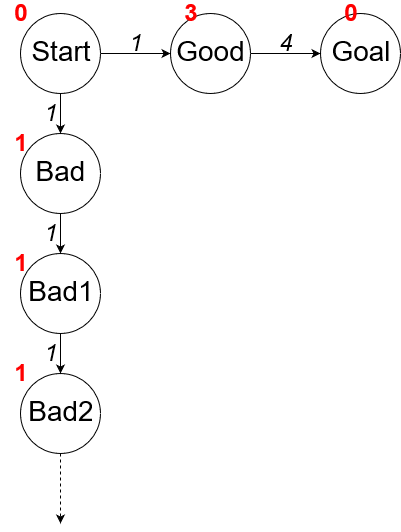
\includegraphics[bb=0 0 401 532,width=0.6\linewidth]{Infinite.png}
\caption{無限ループに陥る状態空間}
\end{figure}


深さ優先探索法に関して、反復深化深さ優先探索とすることにより、先述の状態空間においても解を求めることができるようにした。

\subsection{実装}

\subsubsection{BadNode}

まず、このクラスは、与えられたNodeクラスのサブクラスである。
オーバーライドしたメソッドは以下の1つ。
\begin{itemize}
\item getChildren: Nodeクラスでは内部メンバchildrenを返すが、BadNodeでは新しいBadNodeインスタンスをaddChildしてからchildrenを返す。

\end{itemize}

BadNodeクラスの実装を以下に示す。
\begin{lstlisting}[caption=BadNodeクラス(Search3.java),label=src:BadNode]
    //無限ループを形成するノード
    class BadNode extends Node {

        static int id = 0; //名付け用ID
        BadNode(String theName, int theHValue) {
            super(theName, theHValue);
        }

        @Override
        public ArrayList<Node> getChildren() {
            addChild(new BadNode("Bad" + ++id, hValue), 1); //新しいBadNodeをchildrenに追加
            return super.getChildren(); //childrenを返す
        }
    }
\end{lstlisting}

\subsubsection{深さ優先探索}
深さ優先探索をするdepthFirstメソッドを、以下のように改良した。
\begin{lstlisting}[caption=depthFirstメソッド(Search4.java),label=src:depthFirst]
    /***
     * 反復深化深さ優先探索
     */
    public void depthFirst() {
        ArrayList<Node> open = new ArrayList<Node>();
        open.add(start);
        ArrayList<Node> newOpen = new ArrayList<>(); //深さが1レベル深いオープンリスト
        ArrayList<Node> closed = new ArrayList<Node>();
        boolean success = false;
        int step = 0;

        for (;;) {
            System.out.println("STEP:" + (step++));
            System.out.println("OPEN:" + open.toString());
            System.out.println("NEWOPEN:" + newOpen.toString());
            System.out.println("CLOSED:" + closed.toString());
            // openは空か?
            if (open.size() == 0) {
                //newOpenも空か?
                if (newOpen.size() == 0) {
                    success = false;
                    break;
                }
                //探索を1レベル深くし、newOpenをリセット
                open = newOpen;
                newOpen = new ArrayList<>();
            } else {
                // openの先頭を取り出し node とする.
                Node node = open.get(0);
                open.remove(0);
                // node は ゴールか?
                if (node == goal) {
                    success = true;
                    break;
                } else {
                    // node を展開して子節点をすべて求める.
                    ArrayList<Node> children = node.getChildren();
                    // node を closed に入れる.
                    closed.add(node);
                    // 子節点 m が open にも newOpen にも closed にも含まれていなければ,
                    // 以下を実行.幅優先探索と異なるのはこの部分である.
                    // j は複数の子節点を適切にnewOpenの先頭に置くために位置
                    // を調整する変数であり,一般には展開したときの子節点
                    // の位置は任意でかまわない.
                    int j = 0;
                    for (int i = 0; i < children.size(); i++) {
                        Node m = children.get(i);
                        if (!open.contains(m) && !newOpen.contains(m) && !closed.contains(m)) {
                            // m から node へのポインタを付ける
                            m.setPointer(node);
                            //newOpenに追加
                            if (m == goal) {
                                newOpen.add(0, m);
                            } else {
                                newOpen.add(j, m);
                            }
                            j++;
                        }
                    }
                }
            }
        }
        if (success) {
            System.out.println("*** Solution ***");
            printSolution(goal);
        }
    }

\end{lstlisting}

\subsection{実行例}
BadNodeを用いた状態空間に対し、深さ優先探索、反復深化深さ優先探索、山登り法を実行した結果を以下に示す。

\begin{lstlisting}[caption=深さ優先探索]
(前略)
STEP:848
OPEN:[Bad846(h:1), Good(h:3)]
CLOSED:[Start(h:0), Bad(h:1), Bad0(h:1), Bad1(h:1), Bad2(h:1), (中略), Bad843(h:1), Bad844(h:1), Bad845(h:1)]
STEP:849
OPEN:[Bad847(h:1), Good(h:3)]
CLOSED:[Start(h:0), Bad(h:1), Bad0(h:1), Bad1(h:1), Bad2(h:1), (中略), Bad844(h:1), Bad845(h:1), Bad846(h:1)]
STEP:850
(以下略)
\end{lstlisting}

\begin{lstlisting}[caption=反復深化深さ優先探索]
Depth First Search
STEP:0
OPEN:[Start(h:0)]
NEWOPEN:[]
CLOSED:[]
STEP:1
OPEN:[]
NEWOPEN:[Bad(h:1), Good(h:3)]
CLOSED:[Start(h:0)]
STEP:2
OPEN:[Bad(h:1), Good(h:3)]
NEWOPEN:[]
CLOSED:[Start(h:0)]
STEP:3
OPEN:[Good(h:3)]
NEWOPEN:[Bad0(h:1)]
CLOSED:[Start(h:0), Bad(h:1)]
STEP:4
OPEN:[]
NEWOPEN:[Goal(h:0), Bad0(h:1)]
CLOSED:[Start(h:0), Bad(h:1), Good(h:3)]
STEP:5
OPEN:[Goal(h:0), Bad0(h:1)]
NEWOPEN:[]
CLOSED:[Start(h:0), Bad(h:1), Good(h:3)]
*** Solution ***
Goal(h:0) <- Good(h:3) <- Start(h:0)
\end{lstlisting}

\begin{lstlisting}[caption=山登り法]
(前略)
[Bad199906(h:1)]
[Bad199907(h:1)]
[Bad199908(h:1)]
[Bad199909(h:1)]
(以下略)
\end{lstlisting}

\subsection{考察}
深さ優先探索、山登り法の場合、解(Goal)のほうに進むGoodノードには進まず、解が存在しないがヒューリスティクス関数がより良いBadノードに進んでしまう。しかしながら、反復進化深さ優先探索により、探索するノードの深さを制限することにより、深さ優先探索で探索できない状態空間でも解を求めることができる。


\section{課題1-2}
\begin{screen}
  グループでの進捗管理や成果物共有などについて,工夫した点や使ったツールについて考察せよ.
\end{screen}

課題1-2は実装を伴わない課題であるため、考察のみ記す。

\subsection{考察}
  演習時間内に終わらなかった分は後日全員で集まって課題を進めた。
  連絡手段としてLINEを、ファイル管理にGitHubを用いた。


\end{document}
